
\documentclass[fleqn,12pt]{article}

\usepackage[margin=15mm]{geometry}
\usepackage[utf8]{inputenc}
\usepackage[bulgarian]{babel}
\usepackage[unicode]{hyperref}
\usepackage{amsfonts}
\usepackage{amssymb}
\usepackage{enumitem, hyperref}
\usepackage{upgreek}
\usepackage{indentfirst}
\usepackage{graphicx}

\usepackage{amsmath}
\usepackage{listings}
\usepackage{xcolor}

\definecolor{codegreen}{rgb}{0,0.6,0}
\definecolor{codegray}{rgb}{0.5,0.5,0.5}
\definecolor{codepurple}{rgb}{0.58,0,0.82}
\definecolor{backcolour}{rgb}{0.95,0.95,0.92}

\lstdefinestyle{mystyle}{
    backgroundcolor=\color{backcolour},   
    commentstyle=\color{codegreen},
    keywordstyle=\color{magenta},
    numberstyle=\tiny\color{codegray},
    stringstyle=\color{codepurple},
    basicstyle=\ttfamily\footnotesize,
    breakatwhitespace=false,         
    breaklines=true,                 
    captionpos=b,                    
    keepspaces=true,                 
    numbers=left,                    
    numbersep=5pt,                  
    showspaces=false,                
    showstringspaces=false,
    showtabs=false,                  
    tabsize=2
}
\lstset{style=mystyle}

\graphicspath{ {./img/} }

\title{Тема 22 \\Използване на XML за структуриране, валидация, обработка и представяне на документно съдържание.}

\author{v0.1}
\date{30 юни 2021}

\begin{document}

\maketitle
\tableofcontents
\pagebreak

\section{Добре структуриран XML}

\subsection{Основни концепции}

\textbf{XML таг} наричаме маркер (име на елемент), което е отделено със символите < и >. Примерен таг е \textbf{<hello-world>}.
\bigbreak

\textbf{XML елемент} се състои от отварящ таг, съдържание на елемента и затварящ таг. Примерен елемент е \textbf{<b>how bold of you</b>}.
\bigbreak

\textbf{XML атрибути} наричаме двойки име/стойност, асоциирани с елемент.
Добавят се в отварящия таг със стойности, поставени между ' ' или '' ''.
Тяхната практична стойност е обвързана с конфигурация на елементите.
Пример за поставяне на атрибут е \textbf{<div color='red'></div>}.
\bigbreak

\textbf{XML документ} е текст под формата на един или повече елементи.
\bigbreak

\textbf{XML markup} се състои от всички тагове на даден XML документ.
\bigbreak

\textbf{XML инструкциите} са конструкции предоставящи метаданни на външни приложения. Записваме ги като \textbf{<?$\dots$?>}. Пример за това са инструкциите при php.
\bigbreak

\textbf{XML декларация} наричаме конструкцията \\\textbf{<?xml version='1.0'} \textbf{encoding='UTF-16'} \textbf{standalone='yes' ?>}, която указва версията на XML спецификацията на документа, кодирането на документа и дали е асоцииран с външно DTD.


\subsection{Йерархии}

XML документите могат да имат \textbf{дървовидно} представяне, като отделните възли са XML елементи.
Всеки документ има точно един \textbf{root} елемент, който няма родител, в който се съдържат всички други елементи.

Структурата на XML документите е следната:
\begin{itemize}
    \item \textbf{Пролог} - декларации, стилове и тип на документа;
    \item \textbf{Екземпляр} - конкретна елементна йерархия;
    \item \textbf{Допълнения} - коментари, CDATA секции и инструкции за обработка;
\end{itemize}


\subsection{Синтактични правила}

XML документите трябва да следват следните правила, за да бъдат правилно структурирани:
\begin{enumerate}
    \item \textbf{Затвореност} - всеки отварящ таг трябва да има съвпадащ затварящ таг или да бъде self-closing;
    \item \textbf{Без застъпване} - таговете не могат да се застъпват, като елементите трябва да са подходящо вложени. Некоректно е например \textbf{<a><b></a></b>}.
    \item \textbf{One root to rule them all} - xml документите могат да имат само 1 корен;
    \item \textbf{XML конвенции} - имената на таговете трябва да започват с малка буква, главна буква или ''-'', като не могат да започват с думите xml, XML, Xml, xmL, \dots;
    \item \textbf{Whitespaces} - XML запазва празните пространства в PCDATA;
    \item \textbf{Всеки атрибут трябва задължително да има стойност}, дори и тя да е празен низ;
    \item \textbf{Без запазени XML символи в съдържанието} - те се вмъкват чрез предварително дефинирани entities или \textbf{<![CDATA[\dots]]>} секции.
\end{enumerate}

\subsection{XML пространства от имена}

Пространствата от имена (namespaces) са абстрактна нотация за група от имена.
Едно име може да принадлежи само на едно пространство от имена.
Целта е да се осигури уникалност на имената на XML елементите посредством използването на URI (Uniform Resource Identifier).
За осигуряване на уникалността на префиксите, означаващи пространства от имена се използва само URL (Uniform Resource Locator).
URL не е нужно да е реален, т.е. можем да си използваме каквито си искаме.
\bigbreak
Пространствата от имена за дадена елементна йерархия се задават чрез атрибута xmlns върху корена ѝ, като те важат за всички деца на корена.
Може да съществува едно пространство от имена, наречено такова по подразбиране, което се дефинириа с xmlns без префикс.
Тъй като атрибутите са обвързани с елементите, към които са дефинирани, ако елемент е зададен с префикс на дадено пространство от имена, то не е задължително атрибутите му да са зададени чрез него.

\begin{lstlisting}[language=XML, caption=Doom namespace]
<?xml version="1.0" encoding="utf-8" ?>

<config xmlns="http://config.com" xmlns:doom="http://app.com/myapp">
    <doom:levels>
        <doom:level>
            <doom:npc name="cacodemon" type="regular">
                <doom:count>54<doom:count>
                <doom:power>100<doom:power>
                <doom:health>150<doom:health>
            <doom:npc>
            <doom:npc name="mancubus" type="regular">
                <doom:count>108<doom:count>
                <doom:power>150<doom:power>
                <doom:health>90<doom:health>
            <doom:npc>
        <doom:level>
    </doom:levels>
</config>
\end{lstlisting}


\section{XML валидация чрез Document Type Definitions (DTD)}

\subsection{Цели на валидирането}

Целите на валидацията на XML документите са:
\begin{itemize}
    \item Осигуряване на начин за проверка за коректност на документната структура или съдържание чрез DTD или XML Schema.
    \item Многократно използване на едно описание на документната структура за много XML документи (инстанции на даден документен тип).
    \item Описание на правилата за структуриране на документа, изграждащите го елементи, възможните типове и атрибути и стойностите им по подразбиране.
\end{itemize}


\subsection{DTD структура}

DTD се съхраняват във външни файлове, в самия XML файл или и в двата файла. Състоят се от:
\begin{itemize}
    \item Document Type Definition (DOCTYPE), който информира parser-а, че с документа има асоциирано DTD. Задължително се поставя в началото на документа;
    \item Тяло - съдържа декларациите на елементи, атрибути, entities и нотации;
    \item Затваряне на декларацията на DTD с ];
\end{itemize}

\subsection{Синтаксис}

\begin{lstlisting}[language=XML, caption=Newspaper DTD]

<!-- Document type <!DOCTYPE {name} [...] -->
<!-- Character type <![CDATA [...]]> -->
<!-- Entities <!ENTITY ...> -->
<!-- Notation <!NOTATION {data_type} (PUBLIC|SYSTEM) (PublicID|SystemID)> -->
<!-- Element <!ELEMENT {name} {EMPTY|ANY|type|(child_1, ...))}> -->
<!-- Attribute <!ATTLIST {element_name} {attr_name} {type} {value}> -->
<!-- An attribute type could be 
    - string - CDATA,
    - enumeration - (red|blue|...) 
    - unique id - ID 
    - entity - ENTITY
    ...-->
<!-- An attribute value could be:
    - a default value -> <!ATTRLIST elem name CDATA "blabla">
    - required - #REQUIRED -> <!ATTRLIST elem name CDATA #REQUIRED>
    - optional but with no default value - #IMPLIED -> <!ATTRLIST elem name CDATA #IMPLIED>
    - use only this value - #FIXED -> <!ATTRLIST elem name CDATA #FIXED "constant-value"> -->
<!-- Conditional section <![INCLUDE [...]]>, <![IGNORE [...]]> -->

<!DOCTYPE NEWSPAPER [
    <!ELEMENT newspaper (article+)>
    <!ELEMENT article (headline, body, notes)>
    <!ELEMENT headline (#PCDATA)>
    <!ELEMENT body (#PCDATA)>
    <!ELEMENT notes (#PCDATA)>

    <!ATTLIST article author CDATA #REQUIRED>
    <!ATTLIST article editor CDATA #IMPLIED>
    <!ATTLIST article date CDATA #IMPLIED>

    <!ENTITY newspaper "Vervet Logic Times">
    <!ENTITY publisher "Vervet Logic Press">
    <!ENTITY copyright "Copyright 1998 Vervet Logic Press">

    <!NOTATION jpg PUBLIC "JPG 1.0">
]>
\end{lstlisting}

\section{XML валидация чрез XML Schema}

\subsection{Спецификации}

XML Schema е XML документ, описващ структурата на друг XML документ.
Тя може да се счита за наследник на DTD, предоставящ много по-богати възможности за по-прецизна спецификация на XML структура.

\subsection{Типове данни}

Има две основни групи от типове данни в XML Schema - вградени и дефинирани от потребители.
Вградените са:
\begin{itemize}
    \item примитивни - string, boolean, float, double, ID и др.
    \item производни - language, IDREF и др.
\end{itemize}

Потребителските типове данни се дефинират чрез промяна на съществуващи типове данни чрез определянето на 1 или повече фасети.

\subsection{Фасети}

Фасет е определящ аспект на пространството от стойности за даден тип:
\begin{itemize}
    \item \textbf{Фундаментални фасети (дефинират типа)} - equal, order, bounds, cardinality, numeric;
    \item \textbf{Ограничаващи фасети (ограничават стойностите на типа)} - length, pattern, precision, encoding;
\end{itemize}

\subsection{Структури}


\begin{lstlisting}[language=XML, caption=XSD elements]
<!-- Type definitions -> <simpleType>, <complexType> -->
<!-- Attribute declarations -> <attribute> -->
<!-- Element declarations -> <element> -->
<!-- Attribute group definitions -> <attributeGroup> -->
<!-- Notation declarations -> <notation> -->
\end{lstlisting}

\subsection{Сравнение с DTD}

\begin{itemize}
    \item DTD и XML Schema (или XML Schema Defintion (XSD)) задават правила за структуриране на XML документи;
    \item DTD използва по-стегнат и кратък синтаксис от XSD;
    \item XSD се дефинира на чист XML;
    \item XSD предоставя по-богат набор от възможности за по-строго дефиниране на XML схемата;
\end{itemize}

\section{Алокиране, манипулиране и представяне на XML съдържание}

\subsection{Използване на XSLT (eXtensible StyleSheet Language Transformations)}

XSLT се използва за транслиране на XML документи с помощта на различни стилове и функции.
Резултатът често е някой HTML документ, но може да бъде какъвто и да е текстов файл.
Полезен е когато се разделя презентационния слой на едно приложение от модела на данните му.

XSLT предоставя следните възможности:
\begin{itemize}
    \item Структурни промени на входното съдържание;
    \item Многократно преизползване на елементно или атрибутно съдържание на друго място в документа;
    \item Трансформиране на данни между XML формати;
    \item Определяне на XSL форматиращи обекти и на други средства за представяне на съдържанието в дадена медия (напр. CSS);
\end{itemize}

\begin{lstlisting}[language=XML, caption=XSLT elements]
<!-- Scope of XSLT doc -> <xsl:stylesheet> -->
<!-- Blueprints used in transformation output -> <xsl:template> -->
<!-- Decide which elements to rework -> <xsl:apply-templates> -->
<!-- Evaluate and expression -> <xsl:value-of> -->
<!-- Loop over elements -> <xsl:for-each> -->
\end{lstlisting}

XSLT може да се имплементира в клиентската част на едно приложение (напр. делегация на браузъра или JS) или в сървърната част на едно приложение.
Ако се използва в браузър XML документът се транслира от XHTML.

\subsection{XPath}

XPath служи за адресиране и манипулиране на секции от XML документ.
Използва се при други спецификации като XQL, XSLT и XPointer.
\bigbreak
При XPath коренът на дървото представя целия документ, а не само корена му.
XPath v1.0 се характеризира с това, че:
\begin{itemize}
    \item всеки елемент е възел в XPath дървото;
    \item всеки атрибут е възел в XPath дървото;
    \item текстовия възел представлява текстово съдържание на елемент;
    \item използваните в документа namespace-ове са представени като възли от тип пространство;
\end{itemize}
XPath v2.0 е много по по-богат, по-мощен и по-чувствителен към типа на данните.

\section{Обработка на XML документи}

\subsection{Основни интерфейси и начини на използване на DOM (Document Object Model)}

DOM дефинира логическо дърво, представящо parse-вания XML документ.
Той е стандартизиран начин за достъп до, създаване на и промяна на части от XML документ (напр. елементи, атрибути).

\begin{center} 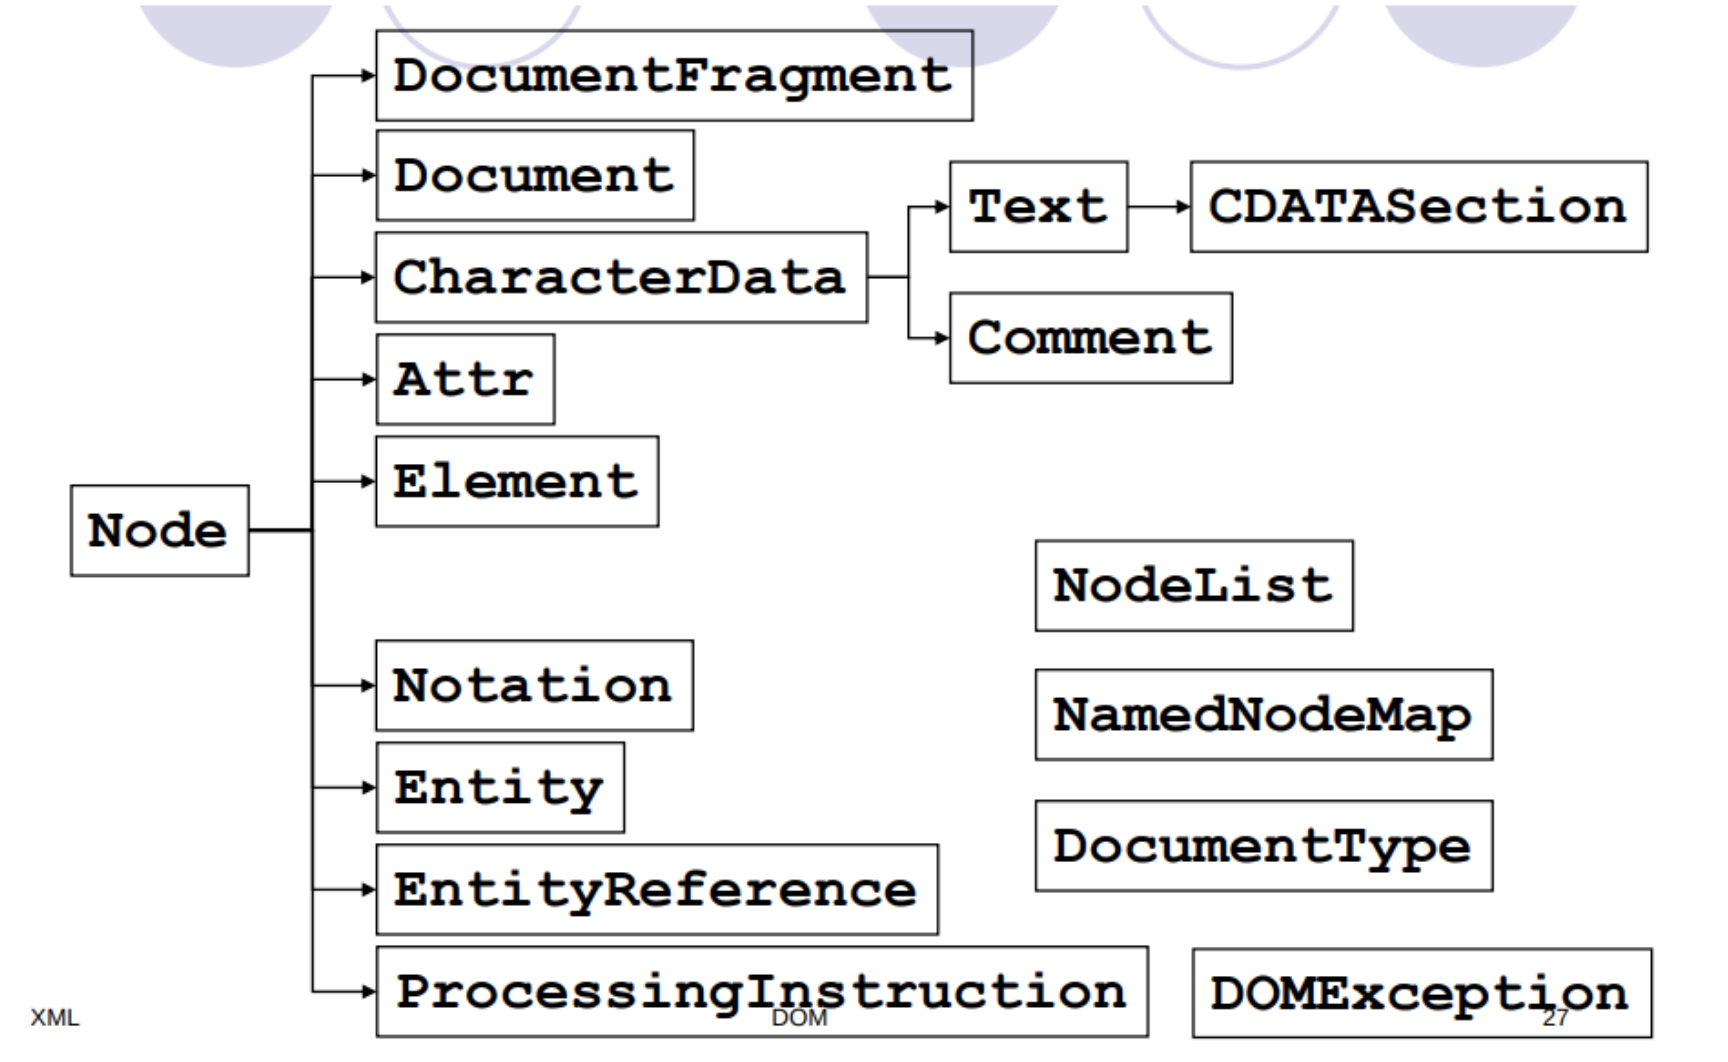
\includegraphics[width=400px]{dom.png} \end{center}

\subsection{Основни интерфейси и начини на използване на SAX (Simple API for XML)}

SAX е event-driven API, който дефинира манипулатори (handlers), съдържащи методи за разбор (push) на XML документа.
Обработката на XML документ от SAX се случва по следния начин:
\begin{itemize}
    \item XML документът се изпраща към SAX parser-а;
    \item XML файлът се прочита ред по ред;
    \item Parser-ът генерира събития (напр. при начало и край на документа, начало и край на елемент, четене на символи и грешки);
    \item При наличие на събитие се използва callback механизъм за извикване на приложението, което имплементира SAX;
\end{itemize}

Дефинира манипулатори (handlers), съдържащи методи за разбор на XML документа (push). С управление по събития (event-driven API) вместо tree-based API.

\subsection{Сравнение между DOM и SAX}

\begin{itemize}
    \item DOM разглежда XML като логическо дърво, докато SAX е базиран на събития.
    \item DOM е добър при обработка на много елементи и структурни промени на документа.
    \item DOM е добър при многократен достъп до XML документа, понеже не се налага да го прочита целия всеки път.
    \item SAX е по-ефикасен за анализ на цели големи документи понеже се налага всеки път да ги прочита целите.
\end{itemize}

\end{document}
